% -- just a two column document
\documentclass[conference]{IEEEtran}

% \usepackage{todonotes}
% \usepackage{cite}
\usepackage{amsmath,amssymb,amsfonts}
\usepackage{algorithmic}
\usepackage{graphicx}
\usepackage{textcomp}
\usepackage{xcolor}
\usepackage{biblatex}
\usepackage{ifthen}
\usepackage{etoolbox}
\usepackage{hyperref}
% \maxdeadcycles=200

\addbibresource{ref.bib}

% Package to count todos

% Counter for todos
\newcounter{todocount}
\setcounter{todocount}{0}

% \todo command
\newcommand{\todo}[1]{
  \stepcounter{todocount}
}

% Display todo count
\newcommand{\showtodocount}{%
  \ifthenelse{\value{todocount}=0}{%
    % No todos
    \section*{Todo List}
    No todos.
  }{%
    % Todos found
    \section*{Todo List}
    Total todos: \arabic{todocount}.
  }
}







\title{Hardware Implementation of MNIST digit recognizer using Binary Neural Networks}





\author{
\IEEEauthorblockN{Joshua Azimullah}
\IEEEauthorblockA{5054354\\
j.r.azimullah@tudelft.nl}
\and
\IEEEauthorblockN{Pieter Becking}
\IEEEauthorblockA{4685377\\
PBecking@tudelft.nl}
\and
\IEEEauthorblockN{Christian van den Berg}
\IEEEauthorblockA{00000000\\
email@example.com}
\and
\IEEEauthorblockN{Ioannis Karydis}
\IEEEauthorblockA{5954460\\
ikarydis@tudelft.nl}
}

\begin{document}
\maketitle


\begin{abstract}
\end{abstract}

\todo{general todos}
\todo{work out all todos}
\todo{Each section in the beginning describes what it will say}
\todo{Connecting signal words?}


\section{Introduction}

\subsection{Basic Theory of Binary Neural Networks}


\todo{rewrite this academically}
BNN are the ultimate quantization method for neural networks. There is no way of quantizing a weight to lower than 1-bit. Quantizing to 1-bit opens up a unique new way of computation, since instead of any other number of bits representation, 1-bit multiplicaiton with 1-bit produces only 1 bit. Therefore a multiplicaiton can be modelled as a truth table. This opens the possibility of many hardware efficiency improvements over traditional quantized and floating-point neural nets.


Overall, BNNs offer a promising approach to developing efficient and high-performance neural networks suitable for a wide range of practical applications.


Binary Neural Networks (BNNs) represent a class of neural networks where weights and activations are constrained to binary values, typically \(\{-1, 1\}\). This binarization facilitates significant computational efficiency, particularly in hardware implementations.

% \subsection{Equivalence of Matrix Multiplication and XNOR-Popcount Operations}

In BNNs, matrix multiplication involving binary weights and activations can be effectively implemented using XNOR and popcount operations in hardware. The XNOR operation provides a binary equivalence to multiplication, while the popcount function, which counts the number of ones in the result, corresponds to the summation step in matrix multiplication. This approach is computationally efficient and well-suited to hardware accelerators.

\todo{these refs}
\todo{ref other section}
This equivalence has been detailed in various studies \cite{placeholder1, placeholder2}, highlighting the advantages of BNNs for high-speed and energy-efficient computations in specialized hardware.




\subsection{Contribution \& Scope of the Project}

\todo{Rewrite aim, such that our aim was to first achieve a respectible accuracy of 95\% on the MNIST dataset, and then further improve the design to optimize on area, power and minimum achievable clock speed.}

\todo{rewrite this part also include: we used mnist dataset (with reference), testset of 10.000 images. }

It covers both training and inference phases, providing a complete view of the BNN's practical use and performance.

\subsection{Outline}

\todo{written table of contents for coming sections}

\section{Overview of BNN Architecture}

\subsection{Training Architecture}
Section \autoref{ref:why_768} provides a rationale for choosing 768 input values over 784, demonstrating superior performance in our specific context.

The architecture of our training network is outlined as follows:
\begin{itemize}
    \item The input vector consists of 768 values, each either -1 or 1.
    \item The first layer performs a matrix multiplication using a weight matrix of size \(1024 \times 768\).
    \item A hardtanh activation function is applied, resulting in output values constrained within the range \(\{-1, 1\}\).
    \item The second layer performs a matrix multiplication with a weight matrix of size \(10 \times 1024\).
    \item The resulting output vector comprises 10 summed values.
    \item The maximum value among these 10 sums is selected as the prediction.
\end{itemize}

\subsection{Inference Network Architecture}
The inference network shares the same mathematical structure as the training network. The primary difference lies in the activation function: the inference network employs a hard activation to constrain outputs strictly to -1 and 1.



\section{Implementation of BNN architecture}
\subsection{Software implementation}
Our Binary Neural Networks (BNNs) are trained using PyTorch, leveraging the Adam optimizer and CrossEntropy loss function, with one-hot encoded outputs. Prior to training, the input values are rounded to \(\{-1, 1\}\), ensuring the network adapts to these binary inputs. Training is conducted in floating-point representation, with binarization applied post-training.

In the MNIST dataset, the 8-bit input values are pre-processed such that values are mapped to $1$ if $\geq 128$, and to $-1$ otherwise. The HardTanh function is used during training to nudge activations towards hard binary values. 

Parallel evaluations using NumPy, simulating the potential BNN's performance, involve rounding matrices to \(\{-1, 1\}\) to validate that inference based on the matrix multiplications using the rounded values aligns with the outcomes predicted by the PyTorch model.


\subsection{Hardware implementation}

% \todo{add in actual hardware architecture}
% \todo{image}
% \todo{xnor\_popcount}
% \todo{matrix\_2}
% \todo{memory}
% insert images here that show the hardware architecture of the xnor popcount and matrix 2
% first figure overview.pdf
% next figure Xnor_popcount.pdf
% next figure majority_classifier.pdf

% \todo{section on hardware architecture}
% \todo{ref to appendix label:xnor\_maths}
% \todo{csa adder tree popcount}
% \todo{matrix2 counter network:}
% \todo{approach 10 counters and finding highest using tree compare}

% \subsection{Hardware implementation}
% Figrue \ref{fig:overview} shows the overall hardware architecture of the BNN.


% The XNOR Popcount Evaluator, shown in Figure \ref{fig:xnor_popcount}, represents the first matrix multiplication and the hard activation after.
% The Majority Classifier, shown in Figure \ref{fig:majority_classifier} represents the second matrix multiplication and the final determining of the output prediction by choosing the highest sum

% each clock cycle both a row of the first matrix multiplication in xnorpopcount and a column of the second matrix in majority classifier are processed in parallel. The bottleneck in this process is the xnorpopcount so it doesn't make sense to do the second matrix faster. the second matrix is in hardware done by just 
% each cycle the xnor popcount decides if the (with matrix 1 row xnorred) vector has a popcount greater than or equal to 384, then this bit is used, in the majority classifier, to xnor with the matrix 2 weight column which produces a 10 bit vector. inside the majority classfier each bit that is 1 their respective counter will increase. the prediction result is a 10 bit vector which is all 0 excpet 1 on the place of the respective counter which is the highest of all



% in the beginning on reset both the matrix\_1 and matrix\_2 counts are reset to 0

% the matrix\_1 and 2 counts, shown in overview, are used to specify the current row in the matrix 1 and 2 register files.
% matrix 1 count is always increased each clock cycle until it reaches the end of the register file, 

% The XNOR popcoutne evaluator takes as input both the input vector and the current weights\_1 row. these togheter are xnorred and popcounted which is the same as a dot product shown in \ref{appendix:bnn_maths}, this evaluator outputs 1 bit : is this sum is greater than or equal to 384. also it outputs an is valid bit that start with 0 which is just a lfsr counter that can count until n, if it is n it will always output 1. given the optimization described in \ref{ref:pipeline_popcount}, the popcount sum is not always valid, but will be valid after n cycles depending on the optimization.

% next the majority classifier which will enable if the is valid is set. also if is valid is set the matrix 2 count will increase after a cycle, this means that majority classifier matrix 2 count lags behind the xnor popcount matrix 1 count by the number of cycles it takes for the xnor popcount to set the is valid high after a reset
% no additional enable is needed as a rst to 0 means that the device start predicting
% the majority classifier (not shown on the image) also holds a count (which is just the same as matrix 2 count) and if that count is equal to the hidden size, the done flag is set high and the device has finished it's prediction

% \subsection{Hardware Implementation}

\autoref{fig:overview} shows the hardware architecture of the Binary Neural Network (BNN). 

The XNOR Popcount Evaluator (\autoref{fig:xnor_popcount}) performs the first matrix multiplication and activation by XNORing and popcounting the input vector with the current row of weights. It outputs a bit indicating if the sum is $\geq 384$. The Majority Classifier (\autoref{fig:majority_classifier}) conducts the second matrix multiplication, determining the output by choosing the highest sum among the columns.

In each clock cycle, a row from the first matrix (XNOR Popcount) and a column from the second matrix (Majority Classifier) are processed in parallel. The XNOR Popcount Evaluator is the bottleneck, so the second matrix operation isn't accelerated. 

On reset, both matrix\_1 and matrix\_2 counters reset to 0. These counters, as shown in \autoref{fig:overview}, select the current row and column in the respective matrix register files. The matrix\_1 counter increments each cycle until it completes the register file. 

The XNOR Popcount Evaluator takes the input vector and the current row from weights\_1, XNORs them, and popcounts the result, outputting a bit if the sum $\geq 384$. It also produces a validity bit, initially set low, which counts to a specific count $n$ using an LFSR counter, after which it is set high. This bit is set after $n$ cycles based on the optimization in Section \ref{ref:pipeline_popcount}.

The Majority Classifier activates if the validity bit is set. Upon activation, it increments the matrix\_2 counter after each cycle, resulting in a delay behind the matrix\_1 counter by $n$. No additional enable signal is needed; a reset to 0 starts the prediction process directly. The Majority Classifier also holds a count equivalent to the matrix\_2 count, and when this count equals the hidden size $1024$, the done flag is set high, signaling prediction completion.




\begin{figure}[h]
    \centering
    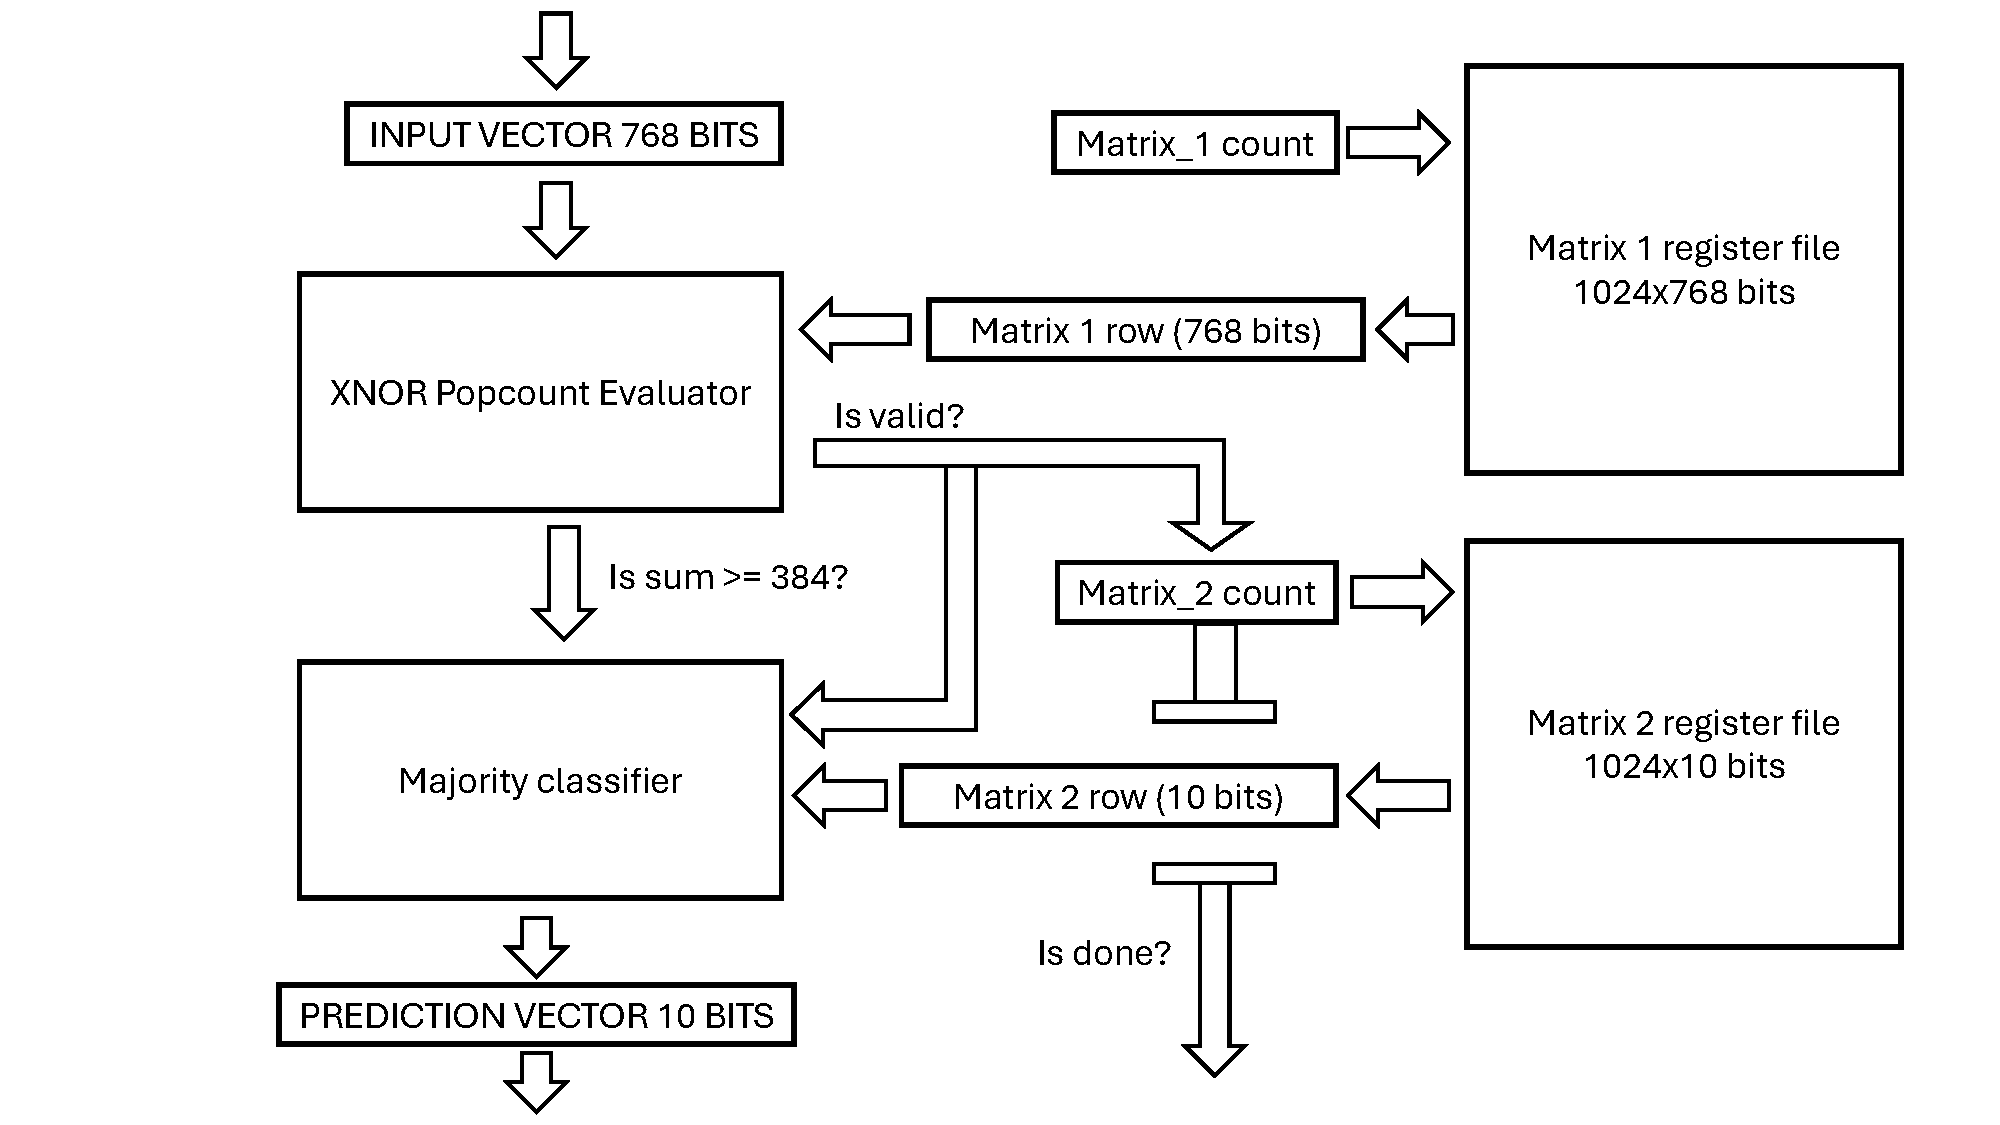
\includegraphics[width=0.4\textwidth]{overview.pdf}
    \caption{Overview of the hardware architecture.}
    \label{fig:overview}
\end{figure}

\begin{figure}[h]
    \centering
    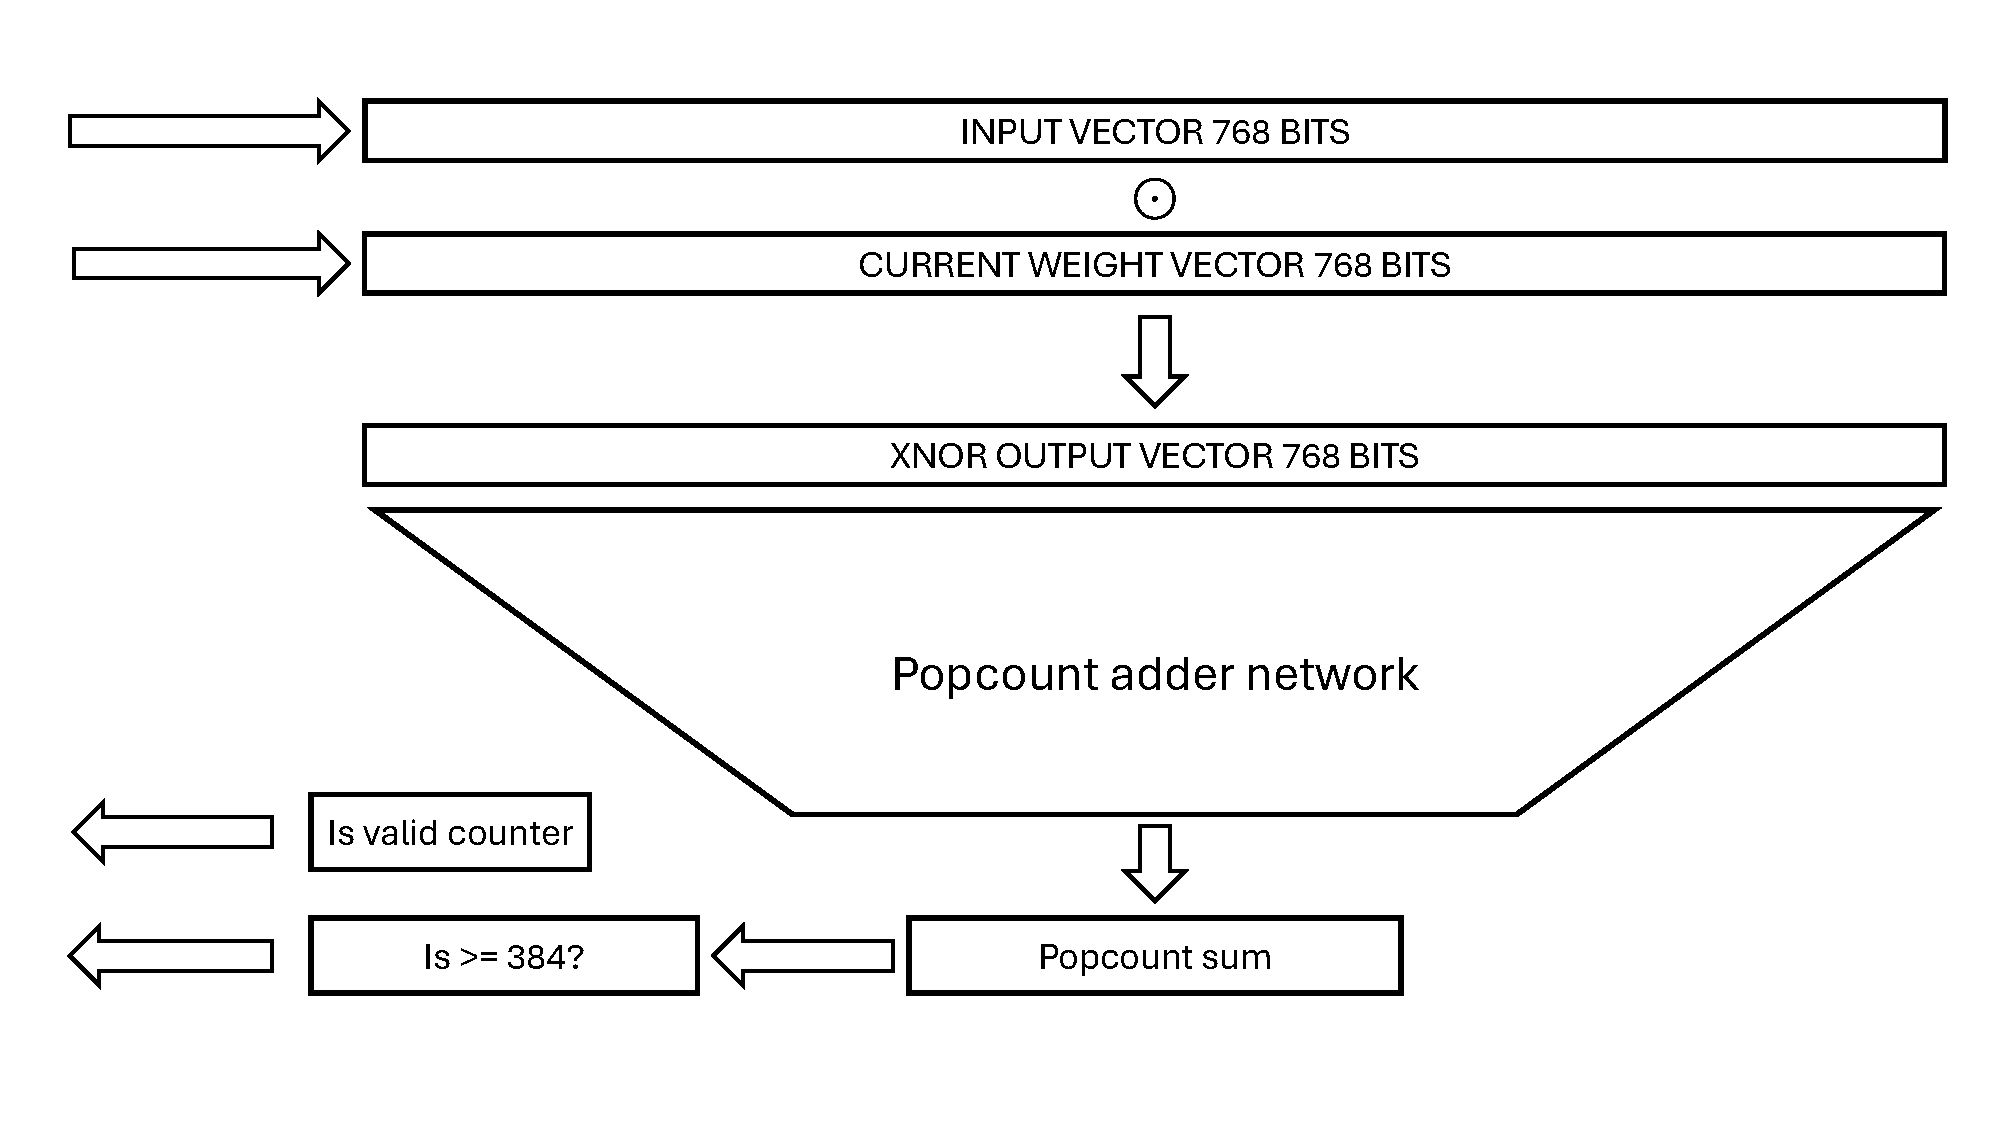
\includegraphics[width=0.4\textwidth]{Xnor_popcount.pdf}
    \caption{XNOR Popcount Evaluator.}
    \label{fig:xnor_popcount}
\end{figure}

\begin{figure}[h]
    \centering
    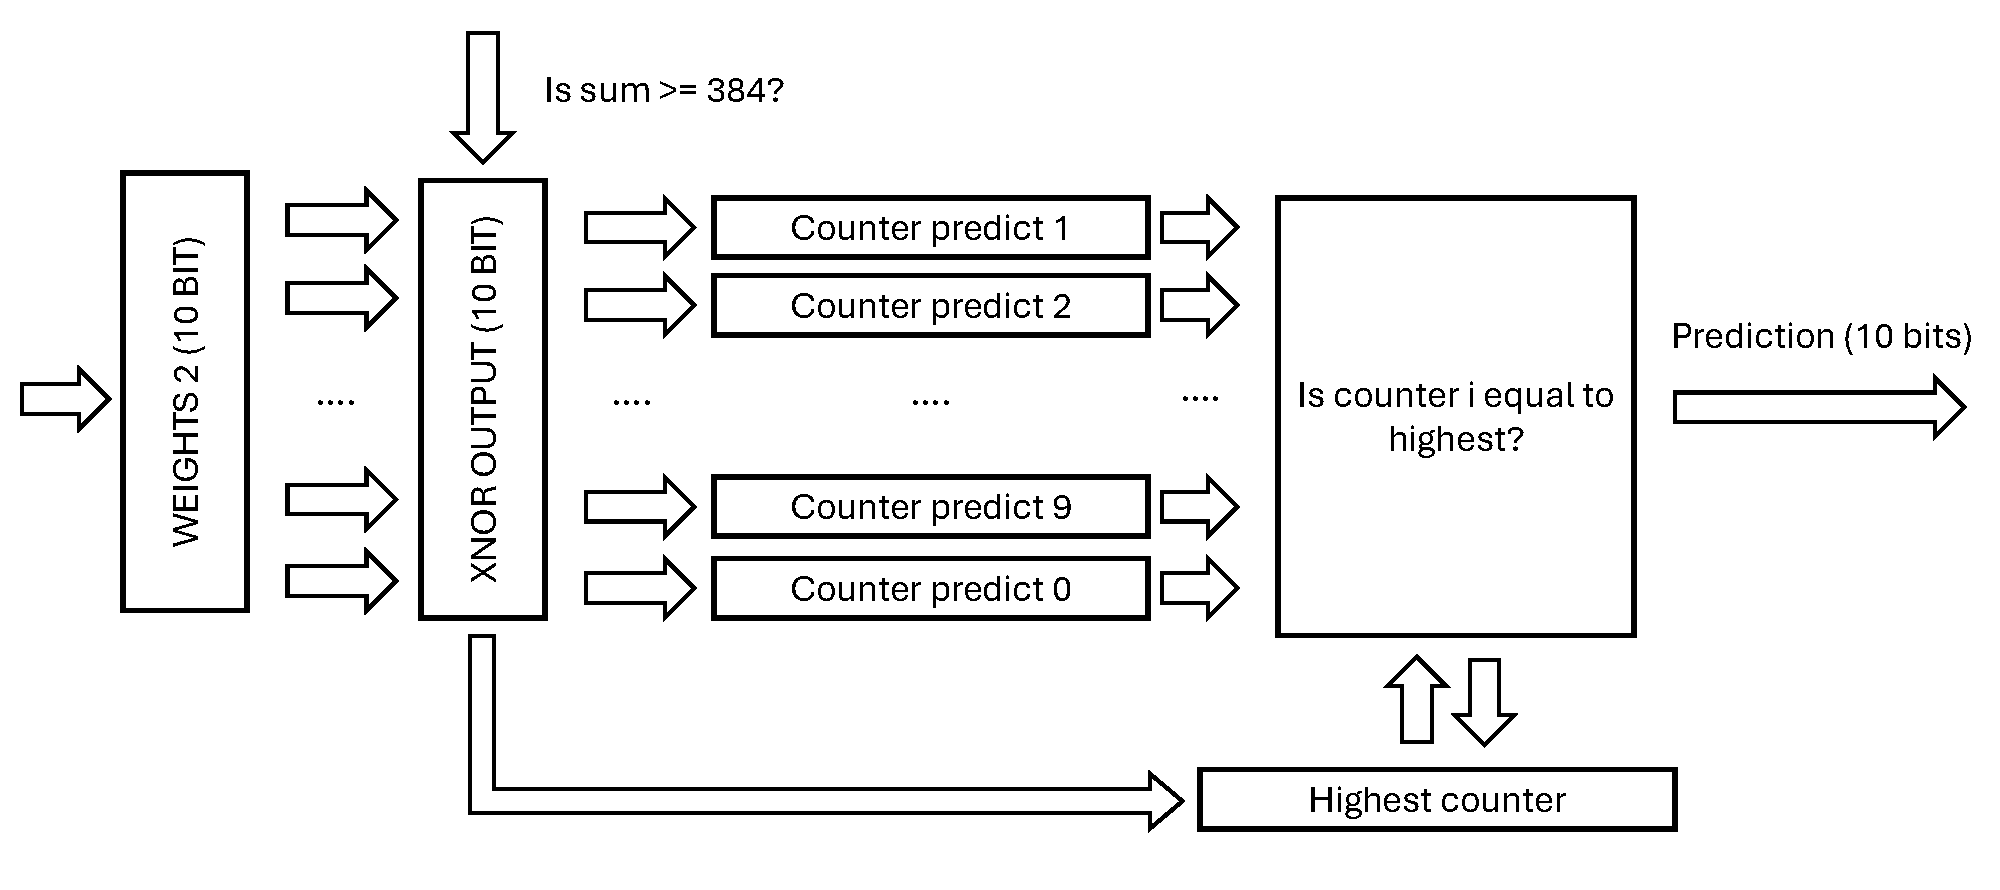
\includegraphics[width=0.4\textwidth]{majority_classifier.pdf}
    \caption{Majority Classifier.}
    \label{fig:majority_classifier}
\end{figure}





% \subsection{Optimizations}
% \subsubsection{Pipelining popcount}
% \label{ref:pipeline_popcount}
% the popcount could of course be done within one clock cycle using a large csa network, but in Section \ref{ref:exploration_pipelining} we did an exploration of different number of pipelined registers in between the adder network. From that 4 levels was chosen as the best number of levels, there for only after $n=4$ cycles the popcount sum is the actual sum, after which each cycle a new valid sum is produced. 

% \subsubsection{Majority classifier only LFSR counters}
% while at first we did a counter for each digit to be classified and later comparing those counts in a tree structure to show which one is highest. it isn't actually necessary to have this tree after if the "highest count" is kept during counting. This highest counter is connected to all other counters showing if it is equal to the highest. if some counter will increase AND it is equal to the highest counter, the highest counter will increase as well.

% Now since the counters don't need to actually compare, real counts don't need to be kept: this opens up the possibility to replace all counters with an lfsr counter instead providing the same function


\subsection{Optimizations}
\subsubsection{Pipelining Popcount}
\label{ref:pipeline_popcount}

Instead of performing the popcount in a single clock cycle using a large Carry-Save Adder (CSA) network, our exploration in \autoref{ref:exploration_pipelining} determined that a pipelined approach with four registers between the adder stages is optimal. Thus, the popcount result becomes valid after $n=4$ cycles, with subsequent cycles producing new valid sums.

\subsubsection{LFSR-Based Majority Classifier}

Initially, individual counters for each digit were used, along with a tree structure to identify the highest count. However, this structure is redundant if the highest count is tracked dynamically. Each counter is compared against the current highest count. If a counter matches the highest count and is to be incremented, the highest count is updated accordingly. This update is achieved by performing a bitwise AND operation between a 10-bit vector indicating counters equal to the highest count and a 10-bit vector indicating counters to be incremented. An OR reduction of this resultant vector determines if the highest count should increase. 
Ultimately, this approach allows the additional optimization of replacing normal counters with Linear Feedback Shift Register (LFSR) counters, which provide equivalent functionality using less area.








\section{Results}

% \todo{section on testing methodology}
% \todo{split into three parts}

% \todo{testing individual parts using fake generated data}

% \todo{subsection testing using ghdl technology for rapid iteration}

% \todo{final testing whole network using all 10.000 test images}
\subsection{Simulation Setup}

The initial model, developed in PyTorch, was translated into raw NumPy operations using values of 1 and -1. Upon validation, the NumPy implementation was segmented into the XNOR Popcount and Majority Classifier components.

This segmentation allowed the generation of random test data for both components, output as binary text files containing 0s and 1s. These text files served as inputs for testbenches to validate the functionality of each component individually.

Additionally, text files for input vectors and corresponding labels were generated using the same method. This enabled testing the entire 10,000-image MNIST testset to verify the device's operation.

Simulations were executed using GHDL to accelerate the simulation process and facilitate rapid testing iterations.



\subsection{Demonstration}
\todo{Demonstration show accuracy from simulation}



\subsection{Design metric results}

\todo{subsection accuracy}
\todo{subsection area}
    \todo{XNOR Popcount Evaluator}
    \todo{Majority Classifier}
    \todo{memory}
\todo{subsection power}
    \todo{XNOR Popcount Evaluator}
    \todo{Majority Classifier}
    \todo{memory}
\todo{subsection timing}
    \todo{XNOR Popcount Evaluator}
    \todo{Majority Classifier}
    \todo{memory}

\subsection{General design Trade-Off}

\todo{section on hardware possible strategies}
\todo{subsubsection strategy do everything sequentially}
\todo{subsubsection strategy do everything in parallel in one tick}
\todo{subsubsection strategy mixed approach, since parallel would be huge and sequentially would be unneccesary slow for little area and power gains due to weights storage that is mandatory}

\subsection{Hardware Trade-off Results}

\subsubsection{Small section that weight memory is most of the area}
	% - [ ] full design
	% 	- [ ] note on how memory is most of the area
\subsubsection{XNOR popcount}
\label{ref:exploration_pipelining}
\todo{Explanation of results:}
\todo{0 levels and 1 levels a wide number of valid divisors of 768 were tested and shown her}
\todo{2 and 3 levels have too large exploration space thus first a reasonable setup was chosen and then for each additional test, only the part where the lowest slack was changed}
	% - [ ] xnor popcount exploration
	% 	- [ ] direct csa tree
	% 	- [ ] 1 level
	% 	- [ ] 2 levels
	% 	- [ ] 3 levels
 
\subsubsection{Matrix 2}
	% - [ ] matrix_2_design
\todo{One line of original with real adders}
\todo{One line of improved with lfsr counters}


\subsection{Accuracy Trade-Off}

\todo{why not CNN decision: would probably require somewhere a linear layer anyways, or a large number of layers vastly reducing speed}

\todo{somewhere needs to be put a better reasoning why 2 matrices are more efficient: either have 1024 counters = excesive or 1024x768 counts which is slow and area gains are low}
The initial goal of our Binary Neural Network (BNN) architecture was to achieve a high level of performance using a single matrix for computations. However, this approach did not meet the target accuracy of 95\%, necessitating exploration of alternative designs.


Subsequent experiments with two matrices in the network structure suggested that this configuration could offer a similar level of computational efficiency while potentially improving accuracy. 

\textit{Results pending. This section will present accuracy metrics for different network configurations once available.}

\todo{lower hidden size, would drop accuracy too much}
\todo{lower input size also}


\label{ref:why_768}
To further optimize the input dimensions, we reduced the number of inputs from 784 to 768 by dropping the last 16 inputs. This simplification leverages the powers of two, specifically \(768 = 512 + 256 = 2^9 + 2^8\), which can simplify the hardware and align more efficiently with binary operations. This reduction did not impact performance.


 








\section{Conclusions}
\todo{it was less area than matrix multiplication lab-1}
\todo{timing bottleneck mostly from memory}

\todo{future work}
\todo{subsection better memory library}
\todo{subsection other problems}
\todo{subsection double is done}



\appendix

\section{Mathematical Foundations for Hardware Implementations}

\label{appendix:bnn_maths}

\subsection{First matrix multiplication with activation}

This section demonstrates that performing matrix-vector multiplication followed by a hard activation is equivalent to using XNOR operations, popcount, and a subsequent comparison.
The matrix-vector multiplication \(\mathbf{A} \mathbf{b}\) shown in Equation \ref{eq:matrix_vector_multiplication} results in a vector \(\mathbf{c}\). Each element \(c_i\) of this vector is obtained by the dot product of the \(i\)-th row of matrix \(\mathbf{A}\) with vector \(\mathbf{b}\), as described in Equation \ref{eq:dot_product}. This can be further expanded into component-wise multiplication and summation (Equation \ref{eq:component_wise_dot}). When elements \(a_{ij}\) and \(b_j\) are binary (\(1\) or \(-1\)), we map them to \(1\) and \(0\) respectively, as shown in Equation \ref{eq:mapping}, enabling the use of XNOR for the multiplication, as described in Equation \ref{eq:xnor}.

\begin{figure}[h]
    \centering
    \begin{equation}
    \mathbf{c} = \mathbf{A} \mathbf{b}
    \label{eq:matrix_vector_multiplication}
    \end{equation}

    \begin{equation}
    c_i = \sum_{j=1}^n a_{ij} b_j
    \label{eq:dot_product}
    \end{equation}

    \begin{equation}
    c_i = \sum_{j=1}^n (a_{ij} \cdot b_j)
    \label{eq:component_wise_dot}
    \end{equation}

    \begin{equation}
    a'_{ij} = \begin{cases}
    1 & \text{if } a_{ij} = 1 \\
    0 & \text{if } a_{ij} = -1
    \end{cases}, \quad
    b'_j = \begin{cases}
    1 & \text{if } b_j = 1 \\
    0 & \text{if } b_j = -1
    \end{cases}
    \label{eq:mapping}
    \end{equation}

    \begin{equation}
    a_{ij} \cdot b_j = \text{XNOR}(a'_{ij}, b'_j)
    \label{eq:xnor}
    \end{equation}

    \caption{Matrix-vector multiplication and equivalent dot product representation.}
    \label{fig:matrix_vector_multiplication}
\end{figure}


\begin{figure}[h]
    \centering
    \begin{equation}
    c = \sum_{i=1}^n a_i b_i
    \label{eq:dot_product_sum}
    \end{equation}

    \begin{equation}
    c = \left|\{c_i \mid c_i = 1\}\right| - \left|\{c_i \mid c_i = -1\}\right|
    \label{eq:dot_product_count}
    \end{equation}

    \begin{equation}
    |\{c_i \mid c_i = -1\}| = n - |\{c_i \mid c_i = 1\}|
    \label{eq:negative_count}
    \end{equation}

    \begin{equation}
    a \cdot b = 2 \left|\{c_i \mid c_i = 1\}\right| - n
    \label{eq:dot_product_simplified}
    \end{equation}

    \begin{equation}
    \text{activation}(c) = \begin{cases}
    1 & \text{if } 2 \left|\{c_i \mid c_i = 1\}\right| \geq n \\
    -1 & \text{otherwise}
    \end{cases}
    \label{eq:activation_function}
    \end{equation}

    \begin{equation}
    \text{activation}(c) = \begin{cases}
    1 & \text{if } \left|\{c_i \mid c_i = 1\}\right| \geq \frac{n}{2} \\
    -1 & \text{otherwise}
    \end{cases}
    \label{eq:activation_function_half}
    \end{equation}

    \begin{equation}
    \text{activation}(a \text{ XNOR } b) = \begin{cases}
    1 & \text{if } \text{popcount}(a \text{ XNOR } b) \geq \frac{n}{2} \\
    -1 & \text{otherwise}
    \end{cases}
    \label{eq:activation_xnor}
    \end{equation}

    \caption{Dot product calculation and activation function.}
    \label{fig:dot_product_activation}
\end{figure}

In Figure \ref{fig:dot_product_activation}, Equation \ref{eq:dot_product_sum} sums the products of the components. Equation \ref{eq:dot_product_count} translates the sum into a count of \(1\)s and \(-1\)s. The total count of \(-1\)s can be expressed as the complement of the count of \(1\)s (Equation \ref{eq:negative_count}). The dot product simplifies to Equation \ref{eq:dot_product_simplified}. The activation function (Equation \ref{eq:activation_function}) sets the output based on the threshold condition, which can also be expressed equivalently as shown in Equation \ref{eq:activation_function_half}. This is related to the XNOR operation in Equation \ref{eq:activation_xnor}, where the activation depends on the population count of the XNOR operation being greater than or equal to half the length of the vector.


\subsection{maths second matrix}
\todo{subsubsection maths is same but now the actual highest popcount needs to be found}





\printbibliography

  \showtodocount

\newpage

\end{document}

